
\documentclass[preprint,12pt]{elsarticle}

\usepackage[spanish]{babel}
\usepackage{amssymb}
\usepackage{graphicx}
\usepackage{float}
\usepackage{lineno}
\usepackage[utf8]{inputenc}
\usepackage{url}
\usepackage{natbib} 
\usepackage{amsmath} 
\usepackage{amssymb} 

\begin{document}
	
	\begin{frontmatter} 

		\title{\huge Gestores de BD NoSQL}
		
		\author{ROBLES FLORES, Anthony Richard     (2016056192))}
		\author{HUICHI CONTRERAS, Franklin Carlos          	(2016054948))}
		\author{PANTY SIHUAYRO, Juan Carlos         	(2015050948))}  
		\author{ATAHUACHI RIVERA, Gabriela Rocío                (2016055341))} 
		\address{Escuela Profesional de Ingeniería de Sistemas}
		\address{Universidad Privada de Tacna}
		\address{Tacna, Perú}
		
%% ABSTRACT --------------------------------------------------------------------------------------------------------------------

		\begin{abstract}
		


		\end{abstract}

%% ----------------------------------------------------------------------------------------------------------------------------------

	\end{frontmatter}

%% RESUMEN ---------------------------------------------------------------------------------------------------------------------

\section{Resumen}
En los últimos años, la cantidad de datos digitales que genera el mundo se ha
multiplicado. Las redes sociales y el cada vez más fácil acceso a Internet del que
disponemos las personas hacen que el volumen de tráfico y de datos que se generan sea
cada vez mayor.
Con el surgimiento de las bases de datos relacionales las empresas encontraron el aliado
perfecto para cubrir sus necesidades de almacenamiento, disponibilidad, copiado de
seguridad y gestión de sus datos.
En este artículo se hablará de los Gestores de Bases de Datos NoSQL y algunas curiosidades.


%% ----------------------------------------------------------------------------------------------------------------------------------


%% INTRODUCION ----------------------------------------------------------------------------------------------------------------

\section{Introducción} 
Son muchas las aplicaciones web que utilizan algun
tipo de bases de datos para funcionar. Hasta ahora
estabamos acostumbrados a utilizar bases de datos SQL
como son MySQL, Oracle o MS SQL, pero desde hace
ya algun tiempo han aparecido otras que reciben el nombre de NoSQL (Not only SQL – No solo SQL) y que
han llegado con la intencion de hacer frente a las bases
relacionales utilizadas por la mayorıa de los usuarios.




%% ----------------------------------------------------------------------------------------------------------------------------------


%% MARCO TEÓRICO ------------------------------------------------------------------------------------------------------------

\section{Marco Teórico}

%% PRIMERA SUBSECCION 

\subsection {\textbf{GESTORES DE BASE DE DATOS}}

\subsubsection{\textbf{NoSQL}}

Las bases de datos NOSQL son un conjunto de bases de datos que no se ajustan al modelo de bases de datos relacionales y sus características.

Estas no tienen esquemas, no usan SQL como el principal lenguaje de consultas, no garantizan la propiedad ACID, los datos almacenados no requieren estructuras fijas como tablas,  normalmente no soportan operaciones JOIN, ni garantizan completamente ACID (atomicidad, coherencia, aislamiento y durabilidad), y habitualmente escalan bien horizontalmente, hacen uso amplio de la memoria principal del computador, resuelven el problema de los altos volúmenes de información y la inmensa cantidad de consultas y transacciones diarias. En resumen, no son relacionales.


%%Ejemplo de cita
\cite{Gartner} 

%%\begin{itemize}
	%%\item x
	%%\item y
	%%\item z
%%\end{itemize}

\subsubsection{\textbf{No SQL otro tipo de Base de Datos}}

Las bases de datos relacionales no tienen nada de malo, pero llegó la web, los servicios en la nube y las aplicaciones con millones de usuarios.
\\
Ante una aplicación con una gran escalabilidad,  las bases de datos pueden llegar a comportarse óptimamente, pero cuanto más crece su estructura y más escalable se quiere hacer un proyecto, más cuesta conseguir que una base de datos relacional sea intuitiva, por no hablar de la dificultad para conservar su simplicidad.

\subsubsection{\textbf{Uso de una base de datos NoSQL}}

En aquellos donde se pueda sacar partido a los puntos fuertes de este tipo de bases de datos. Proyectos en los que se prevea una escalabilidad en un futuro próximo, un gran acceso masivo y cuya estructura y esquemas deban tener grandes cambios para su crecimiento. Proyectos con grandísimas cantidades de información y cuya existencia no tenga sentido de no albergar las ultimas aplicaciones existentes en la web y por lo tanto en continuo cambio.
\\
Un gran proyecto ejemplo de este tipo de bases de datos es Facebook, una web que crece cada día, con una inmensa cantidad de información, con continuas actualizaciones y con un acceso de millones de usuarios al día.


%% SEGUNDA SUBSECCION

\subsection{\textbf{Grandes compañías que utilizan este tipo de bases de datos}}
Son muchas las grandes empresas que hacen uso de este tipo de bases de datos no relacionales, como:
\begin{itemize}
\item Cassandra: Facebook, Twitter…
\item HBase: Yahoo, Adobe…
\item Redis: Flickr, Instagram, Github…
\item Neo4j: Infojobs…
\item MongoDB: FourSquare, SourceForge, CERN… 
\end{itemize}

\subsubsection{\textbf{Su uso es adecuado para aquellas que:}}
\begin{itemize}
\item Manejan volúmenes ingentes de datos
\item Tienen una frecuencia alta de accesos de lectura y escritura
\item Con cambios frecuentes en los esquemas de datos
\item Y que no requieren consistencia ACID
\end{itemize}

\subsubsection{\textbf{Casos de aplicación:}}
\begin{itemize}
\item Servicios Web2.0 (redes sociales, blogs, etc.)
\item Aplicaciones IoT
\item Almacenamiento de perfiles sociales
\item Juegos sociales
\item Gestión de contenidos
\end{itemize}

\subsubsection{\textbf{No adecuados}}
NoSQL no es adecuado para aplicaciones que generen informes
con consultas complejas (necesidad de JOINs), aunque tienen
buena conexión con entornos como MapReduce que permite
paralelizar operaciones complejas como agregaciones, filtros,
etc..

\subsection {\textbf{Bases de datos documentales}}
Una base de datos orientada a documentos está diseñada para gestionar información orientada a
documentos o datos semi-estructurados. Este tipo de bases de datos constituye una de las principales
categorías de las llamadas bases de datos NoSQL.\\
La popularidad del término "base de datos orientada a
documentos"" o "almacén de documentos" ha crecido a la par con el uso del término NoSQL en sí. A diferencia de las conocidas bases de datos relacionales con su definición de “tabla”, los sistemas documentales están diseñados entorno a la definición abstracta de un "documento".\\
Las bases de datos de documentales son consideradas por muchos como un escalón superior ante los
simples gestores de llave-valor, puesto que permiten encapsular pares de llave-valor en estructuras más
complejas denominadas documentos. Por otra parte no existe un esquema estricto a seguir para definir
estos documentos, lo cual simplifica sustancialmente su uso.\\
Almacenar y recuperar todos los datos relacionados como una sola unidad puede entregar ventajas
enormes en el rendimiento y la escalabilidad. De este modo, los gestores de datos no tienen que hacer
operaciones complejas como las uniones para encontrar los datos que normalmente están relacionados,
ya que todo se encuentra en un mismo lugar.
%% Ejemplo de inclusión de imagen
\begin{figure}[H]
	\begin{center}
		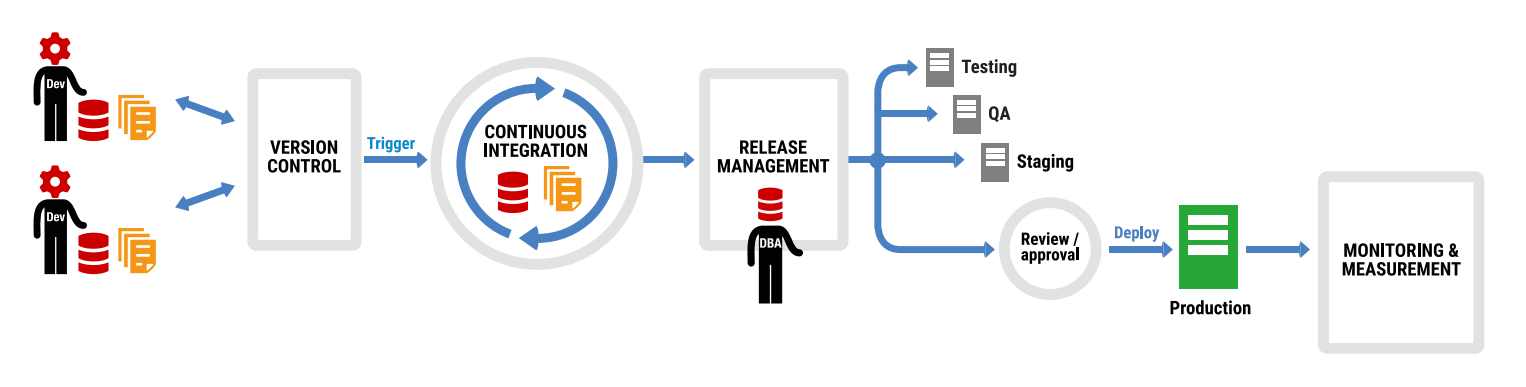
\includegraphics[width=10cm]{./IMAGENES/basededatos_1} 
		\caption{Base de datos documentales}
	\end{center}
\end{figure}
A excepción de algunas, estas bases de datos generalmente proporcionan sus datos a través de HTTP,
almacenan los datos como documentos con la notación de objetos de JavaScript (JSON) y ofrecen
diferentes API para varios lenguajes. Los intereses generales son la sencillez, velocidad y escalabilidad.
Entre las más utilizadas se encuentran: 
\begin{itemize}
\item MongoDB (mongodb.org)
\item CouchDB (couchdb.apache.org)
\item RavenDB (ravendb.net)
\end{itemize}
\begin{figure}[H]
	\begin{center}
		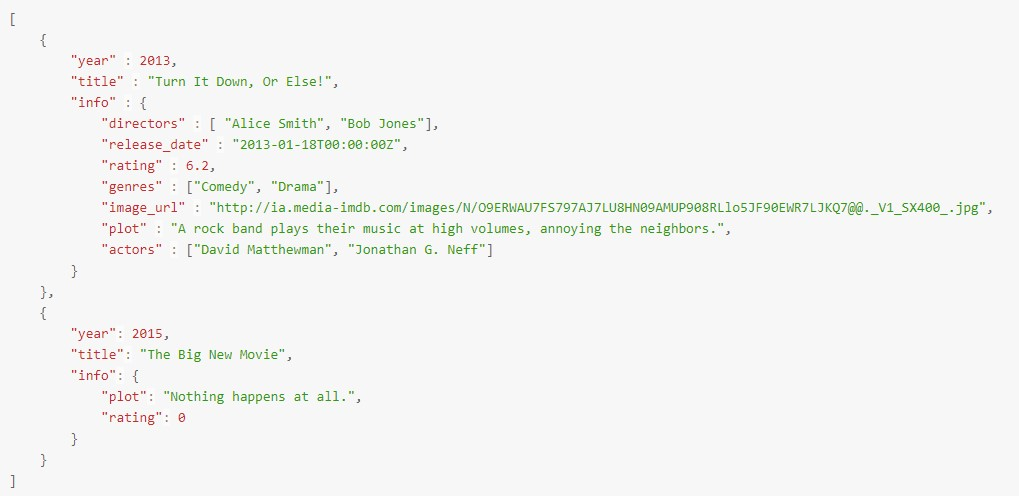
\includegraphics[width=15cm]{./IMAGENES/basededatos_2} 
		\caption{Base de datos documentales}
	\end{center}
\end{figure}


%% ----------------------------------------------------------------------------------------------------------------------------------
 


%% ANÁLISIS ( APLICACIÓN ) ---------------------------------------------------------------------------------------------------

\section{Análisis}

\subsection{\textbf{Análisis 1}}
EDITAR\\

\subsection{\textbf{Análisis 2}}
EDITAR\\

\subsection{\textbf{Análisis 3}}
EDITAR\\

\subsection{\textbf{Análisis 4}}
EDITAR\\

%% ----------------------------------------------------------------------------------------------------------------------------------


%% CONCLUSIONES ---------------------------------------------------------------------------------------------------------------

\section{Conclusiones}

\begin{itemize}

\item Conclusion 1 : \\
Las bases de datos NoSQL son una tecnología muy potente y variada que, si se sabe
emplear de forma correcta, resulta ser una herramienta valiosísima que permitirá
almacenar grandes cantidades de datos y extraer conocimiento de ellos de forma
eficiente, tan necesario hoy en día debido al fenómeno BigData. No en vano, los puestos
profesionales de informáticos que poseen conocimientos sobre alguna de estas
tecnologías se están comenzando a demandar ampliamente.\\

\item Conclusion 2 : \\ 
Estas tecnologías son muy flexibles y versátiles, proponiendo soluciones a problemas
que de otra manera han resultado ser difíciles de abordar. Pero esta tecnología no ha
llegado para reemplazar a las bases de datos relacionales. Los sistemas relacionales
poseen una serie de características y cumplen una serie de requisitos indispensables para
muchos sectores de la informática, como la banca o el comercio electrónico. \\

\item Conclusion 3 : \\ 
Aún quedan muchos aspectos por explorar en esta tecnología, ya que aún no está
madura (es relativamente joven, ya que se comenzó a hablar de ella con fines
comerciales hace poco más de 5 años), faltando todavía experiencia en sistemas en
producción de cara al público. Si se compara con los sistemas relacionales, éstos llevan
solucionando problemas de almacenamiento y securización de datos desde hace más de
50 años.\\

\item Conclusion 4 : \\ 
Las bases de datos NoSQL han llegado para complementar la oferta de bases de datos
de la que se dispone a la hora de abordar los problemas, y en ningún caso es
recomendable alcanzar una posición extrema con respecto a las decisiones que se toman
en este ámbito. Cada problema debe ser analizado en su conjunto, con sus necesidades
particulares para cada caso, y una vez se tiene un esquema claro de esto, se debe buscar
la solución de almacenamiento de entre todas las disponibles que mejor cubra las
necesidades del problema.




\end{itemize}

%% ----------------------------------------------------------------------------------------------------------------------------------

%%  REFERENCIAS BIBLIOGRÁFICAS ------------------------------------------------------------------------------------------
	
	\newpage
	
	\bibliographystyle{apalike} 	%ESTILO
	\bibliography{BIBLIOGRAFIA}	 
	
	
\end{document}
